\subsubsection{Cosine Similarity}

With the cosine based distance, it seems that the fact that the articles are separated into topics makes a better contrast appear between the years. Indeed, because the years are represented by vectors containing the frequencies of the words, and that the dimension of those vectors is reduced by the number of words that are specific for other topics, then if the angle is big, it is due to the language itself and note more on the fact that it can be on opposed subjects.

\begin{figure}[H]
    \begin{minipage}[b]{0.48\linewidth}
        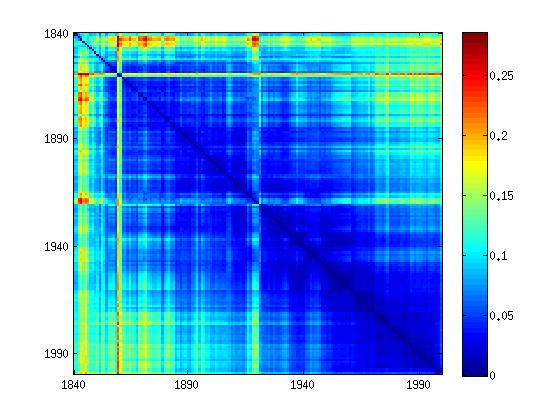
\includegraphics[scale=0.3]{Pictures/topics/cos/topic1.jpg}
        \caption{cosine distance on topic 1: history}
        \label{cos_topic1}
    \end{minipage}\hfill
    \begin{minipage}[b]{0.5\linewidth}
        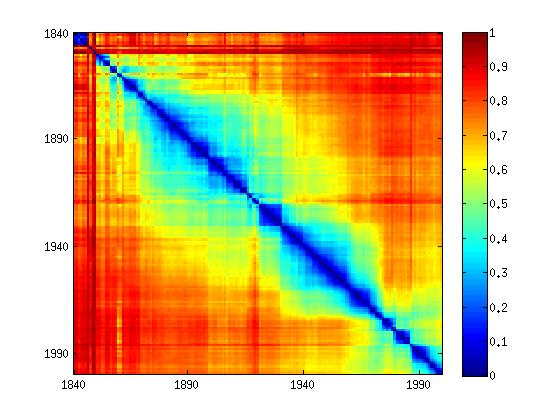
\includegraphics[scale=0.3]{Pictures/topics/cos/topic3.jpg}
        \caption{cosine distance on topic 3: general}
        \label{cos_topic3}
    \end{minipage}\hfill
\end{figure}

There is some topics where we cannot distinguish any drift where an example is shown in figure \ref{cos_topic1}. The concerned topic is about history and religion, so it seems legit that it doesn't change over years and the language drift is hard to enhance for that kind of subject. On the contrary, there is some topics where a drift over years is well marked such as in figure \ref{cos_topic3}. For those cases, the fact that the articles are separated in topics gives an improvement for the cosine metric.

\begin{figure}[H]
    \begin{minipage}[b]{0.48\linewidth}
        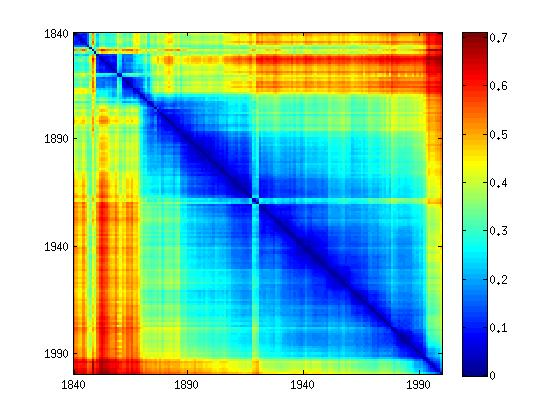
\includegraphics[scale=0.3]{Pictures/topics/cos/topic7.jpg}
        \caption{cosine distance on topic 7: Swiss politics}
        \label{cos_topic7}
    \end{minipage}\hfill
    \begin{minipage}[b]{0.5\linewidth}
        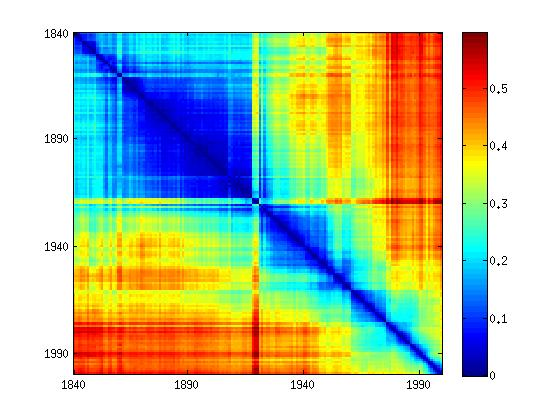
\includegraphics[scale=0.3]{Pictures/topics/cos/topic9.jpg}
        \caption{cosine distance on topic 9: theatre and music}
        \label{cos_topic9}
    \end{minipage}\hfill
\end{figure}

We have also interesting topics such as Swiss politics or music in figures \ref{cos_topic7} and \ref{cos_topic9} where a drift is also enhanced compared to the distance on the whole corpus but the changes are not proportional along the time.